\documentclass[tikz]{standalone}
\usepackage[utf8]{inputenc}

\usepackage{modml}

\tikzset{%
  highlight/.style={rectangle,rounded corners,fill=red!15,draw,fill opacity=0.5,inner sep=0pt}
}
\newcommand{\tikzmark}[2]{\tikz[overlay,remember picture,baseline=(#1.base)] \node (#1) {#2};}
%
\newcommand{\HighlightColumn}[2]{%
    \tikz[overlay,remember picture]{
    \node[highlight,fit=(top#1.north west) (bottom#1.south east)] (#1) {};}
}

\newcommand\sol[1]{\tikz[overlay, remember picture,baseline=-\the\dimexpr\fontdimen22\textfont2\relax]\node[rectangle,fill=blue!50,rounded corners,fill opacity = 0.2,text opacity =1] {$#1$};} 

\begin{document}
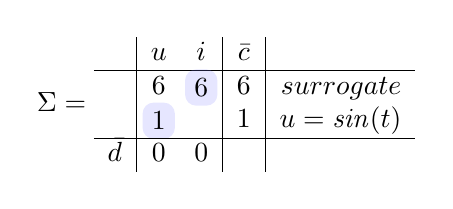
\begin{tikzpicture}
\node(matrix) {
$
\vspace{1.7cm}
  \Sigma = \begin{array}{l|cc|c|r}      
    & u & i & \bar{c} & \\
    \hline
    & 6 & \sol{6} & 6 & \text{surrogate} \\
    & \sol{1} &  & 1 & u = \mathit{sin}(t) \\
    \hline
    \bar{d} & 0 & 0 & 
    \end{array}
\vspace{1.7cm}
$
};
\end{tikzpicture}
\end{document}​
